\documentclass[12pt, a4paper]{article}

\usepackage{hyperref}
\usepackage{mathtools}
\usepackage{graphicx}

\title{Simulation of Two-Phase Flow in Porous Media using a Two-Dimensional Network Model}
\author{Shabbir K.\thanks{Moscow Institute of Physics and Technology}}
\date{\today}


\begin{document}

\maketitle

\section{Volumetric Flow Rate through a cylinder}

Viscous forces act according to:

\[ \frac{F}{A} = \mu \left| \frac{dv}{dr} \right| \]

Where $F$ is the total shearing force on a surface of the layer, this force acts parallel to the surface plane, $A$ is the area of the surface, $\mu$ is the coefficient of viscosity, $v$ velocity of the flow parallel to the plane, and $r$ is the coordinates perpendicular to the plane.

For a cylinder, the volumetric flow rate is given by

\begin{equation} \label{eq:flow-rate}
\boxed{Q = \frac{\pi}{8\mu}\frac{\Delta P}{l} R^4}
\end{equation}


\section{Flow rate in a tube containing meniscus}

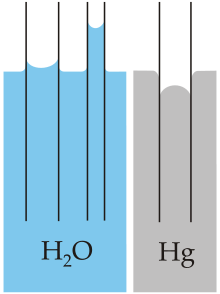
\includegraphics{fig_capact-of-water} \label{fig_capact-of-water}

Figure showing capillary action of water (polar) compared to mercury (non-polar), with respect to a polar surface such as glass (Si–OH). Let us apply this to our case, where the first node is filled with a fluid like water and the second node is filled with a fluid like air, and the our tube is similar to glass. Hence the meniscus will be oriented in a manner shown below.

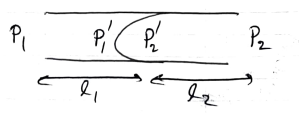
\includegraphics{fig_flowr-1-men}

Let there be a higher pressure in $P_{1}$ than $P_{2}$, the fluid in node which has $P_{1}$ produces a meniscus whose tends move towards the second node. We can break it down into two separate tubes of lengths $l_{1}$ and $l_{2}$, containing fluid of viscosites ${\mu}_1$ and ${\mu}_2$. Then the flow rates for each of the tubes are given by:
\begin{equation} \label{eq:flow-rate-first}
Q_1 = \frac{\pi}{8{\mu}_1} \frac{P_1 - P^{'}_1}{l_1} R_1^4
\end{equation}
\begin{equation} \label{eq:flow-rate-second}
Q_2 = \frac{\pi}{8{\mu}_2} \frac{P^{'}_2 - P_2}{l_2} R_2^4
\end{equation}

Multiplying equations \ref{eq:flow-rate-first} and \ref{eq:flow-rate-second} by ${\mu}_i l_i$
\begin{equation} \label{eq:flow-rate-first-coeff}
Q_1 {\mu}_1 l_1 = \frac{\pi}{8} (P_1 - P^{'}_1) R_1^4
\end{equation}
\begin{equation} \label{eq:flow-rate-second-coeff}
Q_2 {\mu}_2 l_2 = \frac{\pi}{8} (P^{'}_2 - P_2) R_2^4
\end{equation}

Due to continuity, which means no vacuum or fluid can be created, $Q_1 = Q_2$. Since it is the same tube, $R_1 = R_2$. Adding equation \ref{eq:flow-rate-first-coeff} and \ref{eq:flow-rate-second-coeff}, we get:
\begin{equation} \label{eq:flow-rate-intermediate}
Q({\mu}_1 l_1 + {\mu}_2 l_2) = \frac{\pi}{8}R^4(P_1 - P_2 + P^{'}_2 - P^{'}_1)
\end{equation}

In figure \ref{fig_capact-of-water} the water rises because there is a pressure jump at the meniscus, the pressure is lower on the side of the water. Therefore in our case $P^{'}_2 - P^{'}_1$ will have a positive value. Equation \ref{eq:flow-rate-intermediate} becomes:
\begin{equation}
Q = \frac{\pi R^4}{8({\mu}_1 l_1 + {\mu}_2 l_2)}(\Delta P + \frac{2\sigma}{R})
\end{equation}

Let the node on which we are generating linear equations be $N_i$ and the node connected by a tube be $N_j$, if the concave side of the meniscus points towards $N_j$ from $N_i$, then let us say that the meniscus 'points away from $N_i$' or simply 'points away' and in the case of opposite orientation 'points towards'. Let the sign due to the orientation of meniscus be decided by a function called $sigmns(ort, n)$, where $ort$ is the orientation, and $n$ is the number of meniscus in the tube:
\begin{equation}
sigmns(ort, n) = 
\begin{dcases}
-1,&\text{ort points towards, n = 1}\\
0,&\text{n = 0, 2}\\
+1,&\text{ort points away, n = 1}
\end{dcases}
\end{equation}

Finally we get:
\begin{equation} 
Q_{ij} = \frac{\pi R^3}{8({\mu}_1 l_1 + {\mu}_2 l_2)}(R\Delta P_{ij} + 2sigmns(ort, n)\sigma)
\end{equation}

It can be extended to the case when there are more than 1 meniscus, and using $s_{ij}$ for $sigmns_{ij}(ort, n)$:
\begin{equation} \label{eq:flow-rate-main}
\boxed{Q_{ij} = \frac{\pi R_{ij}^3}{8lM_{ij}}(R_{ij}\Delta P_{ij} + 2s_{ij}\sigma)}
\end{equation}

Here
\[ M_{ij} = \sum\limits_{k}{\mu}_{ijk} \frac{l_{ijk}}{l} \]
$Q_{ij}$ is the flow from $N_i$ to $N_j$ and $\Delta P_{ij} = P_i - P_j$. In case, when the flow is in the opposite direction $Q_{ij}$ will take the opposite sign.

\begin{equation}
Q_{ij} = -Q_{ji}
\end{equation}


\section{The linear equations} \label{sec:linear-equ}

Let us apply our method on a simple system consisting of only 5 nodes.

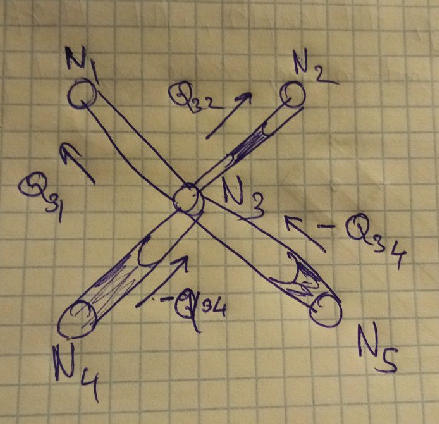
\includegraphics[height=6cm]{fig_simple-5-nodes}

Since there are 4 tubes, we can write 4 equations according to \ref{eq:flow-rate-main}
\[ Q_{31} = \frac{\pi R_{31}^3}{8lM_{11}}(R_{31}\Delta P_{31} + 2s_{31}\sigma) \]
\[ Q_{32} = \frac{\pi R_{32}^3}{8lM_{12}}(R_{32}\Delta P_{32} + 2s_{32}\sigma) \]
\[ Q_{34} = \frac{\pi R_{34}^3}{8lM_{14}}(R_{34}\Delta P_{34} + 2s_{34}\sigma) \]
\[ Q_{35} = \frac{\pi R_{35}^3}{8lM_{15}}(R_{35}\Delta P_{35} + 2s_{35}\sigma) \]

Since the sum of all $Q_{ij}$ is equal to zero. Then as we iterate for each tube connected to the node, in our case we have 4 tubes, it is sufficient to do the following three operations. Here let $K_{ij} = R^3_{ij}/{M}_{ij}$.

\[ [P_i] + R_{ij}K_{ij} \]
\[ [P_j] - R_{ij}K_{ij} \]
\[ [const] - 2s_{ij}\sigma K_{ij} \]
The matrix for Gaussian elimination will be

\[ 
\begin{pmatrix}
	1 & 0 & 0 & 0 & 0 & P_{up}\\
	0 & 1 & 0 & 0 & 0 & P_{up}\\
	-R_{31}K_{31} & -R_{32}K_{32} & (R_{3k}K_{3k} + ...) & -R_{34}K_{34} & -R_{35}K_{35} & -2\sigma(s_{3k}K_{3k} + ...)\\
	0 & 0 & 0 & 1 & 0 & P_{down}\\
	0 & 0 & 0 & 0 & 1 & P_{down}
\end{pmatrix}
\]
 It can be proven that this matrix always has a solution. Once the solution is determined the flow rate can be calculated using equation \ref{eq:flow-rate-main}, and the velocity of flow in each tube is given by
\begin{equation} \label{eq:velocity-in-tube}
\boxed{v_{ij} = \frac{R_{ij}}{8lM_{ij}}(R_{ij}\Delta P_{ij} + 2s_{ij}\sigma)}
\end{equation}

\section{Description of the Model}
The algorithms and methods used to simulate two-phase flow in porous media has many practical applications in oil recovery, hydrology, electricity production where pressurized water is passed through heated pipes and is transformed into steam, etc. Our algorithm presented here is used to find the saturation of a phase with respect to time, the hysteresis curve when the pressure across the porous body is reversed, total capillary pressure as a function of saturation[4], and determination of permeability which appears in Darcy’s law.

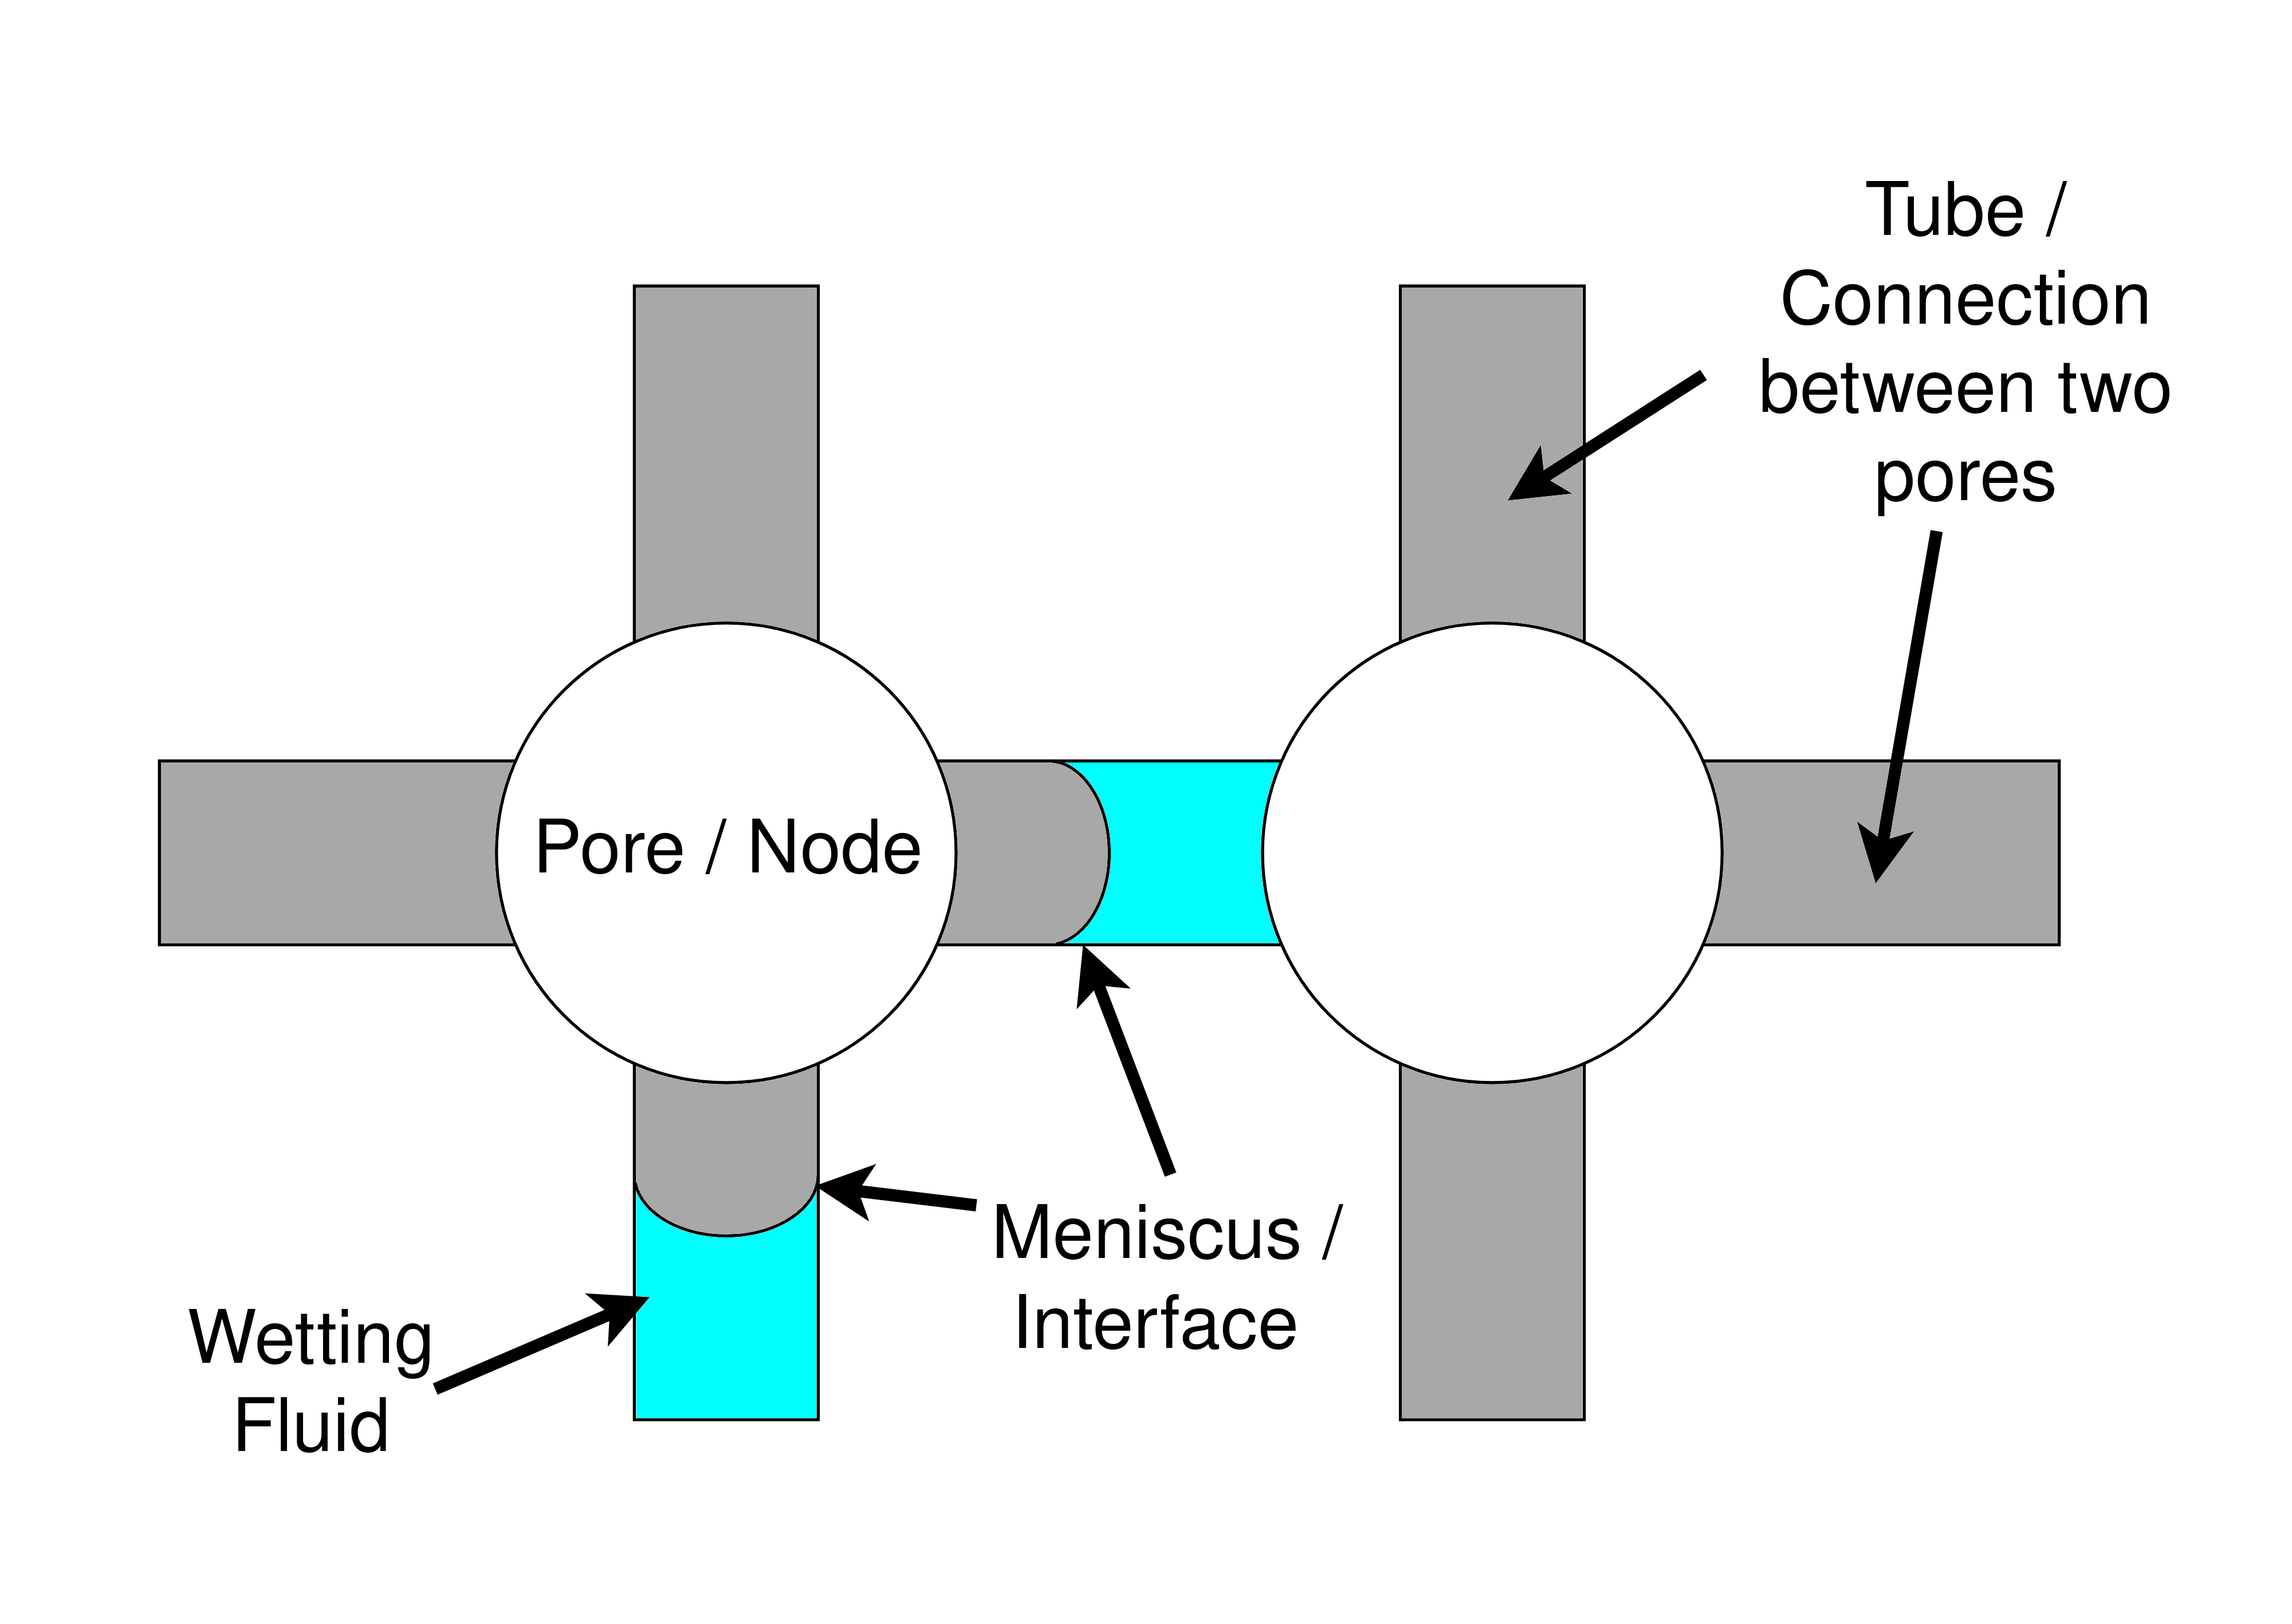
\includegraphics[height=6cm]{fig_descp-of-model}
Figure showing two nodes from the network where the size of the node is much larger than the radius such that the capillary force tends to zero when the meniscus enters a node. 

\section{Algorithm steps}
\begin{enumerate}
	\item \textbf{Input Files:} read input files, radius.txt and mns.txt, mns.txt contains the initial setup of the meniscus
	\item \textbf{Random radius:} add very small random values to the radius, this is done in order to remove the case of two equal radius for simplicity, can be removed later
	\item \textbf{Loop time:} do until a certain proportion of invading fluid is reached for example 0.90:
	\begin{enumerate}
		\item \textbf{Pressure:} determine the pressure at each node using the linear equations given in section \ref{sec:linear-equ}.
		\item \textbf{Velocity:} Calculate the velocity using equation \ref{eq:velocity-in-tube} 
		\item \textbf{time step:} determine the time step, the time step is calculated such that, it is the minimum of the time taken for a meniscus to reach a node it is heading towards. It is calculated by iterating through all the tubes, for a tube the time is determined using the $t_{ij} = x_{ij} / v_{ij}$, here $x_{ij}$ is the distance between the node and and the meniscus closest to it, if the fluid is traveling upwards then it is the node located on the top of the tube, if the velocity is downwards then the node which is at the bottom is used. In case there is no meniscus present, $x_{ij} = l_{ij} / 4$ is used, it is because a meniscus can enter the tube during the time step and this meniscus must not reach the next node, it can happen if the velocity is high and the radius is small. Also if $x_{ij} > l_{ij} / 4$, then $x_{ij} = l_{ij}/4$ is used. This is done in order to smoothen the integration. In the video $l_{ij}/4$ is used, the number can be increased.
		\item \textbf{volume:} The volume displaced in each tube is determined by iterating through all the tubes, $V_{ij} = v_{ij} * t_{min}$.
		\item \textbf{integration:} 
			\begin{enumerate}
			\item \textbf{Store insertion:} create a matrix to store how much of which fluid to insert in each of these tubes.
			\item \textbf{Loop nodes:} Iterate through all the nodes, and for each of the nodes. 
				\begin{enumerate}
					\item divide the tubes into two categories, flow-in-tube - here the fluid from these tubes flow into the nodes, flow-out-tubes here we insert the fluid into the tube from the node
					\item Find out the total of fluid1, fluid2, which is the total of each fliud from all flow-in-tubes.
					\item Start filling the each of the flow-out-tubes where the flow will go into in ascending order of the radius of the tube. This will be done simply be adding the quantity of fluid1 and fluid2 to the matrix created above.
					\item while filling fist use fluid1, once fluid1 is used up then start using fluid2, which means if in a tube we have to insert two fluids, then fluid1 will go in first.
				\end{enumerate}
			\item \textbf{Fluid addition:} For each of the tubes, add the volume of fluid determined to be added. After addition if there are more than 2 meniscus, then merge them retaining their center of masses.
			\end{enumerate}
		\item \textbf{Picture:} Save a picture of the current configuration.
		\end{enumerate}
	\item {Video:} Make a video file from the pictures.
\end{enumerate}

\section{Results}
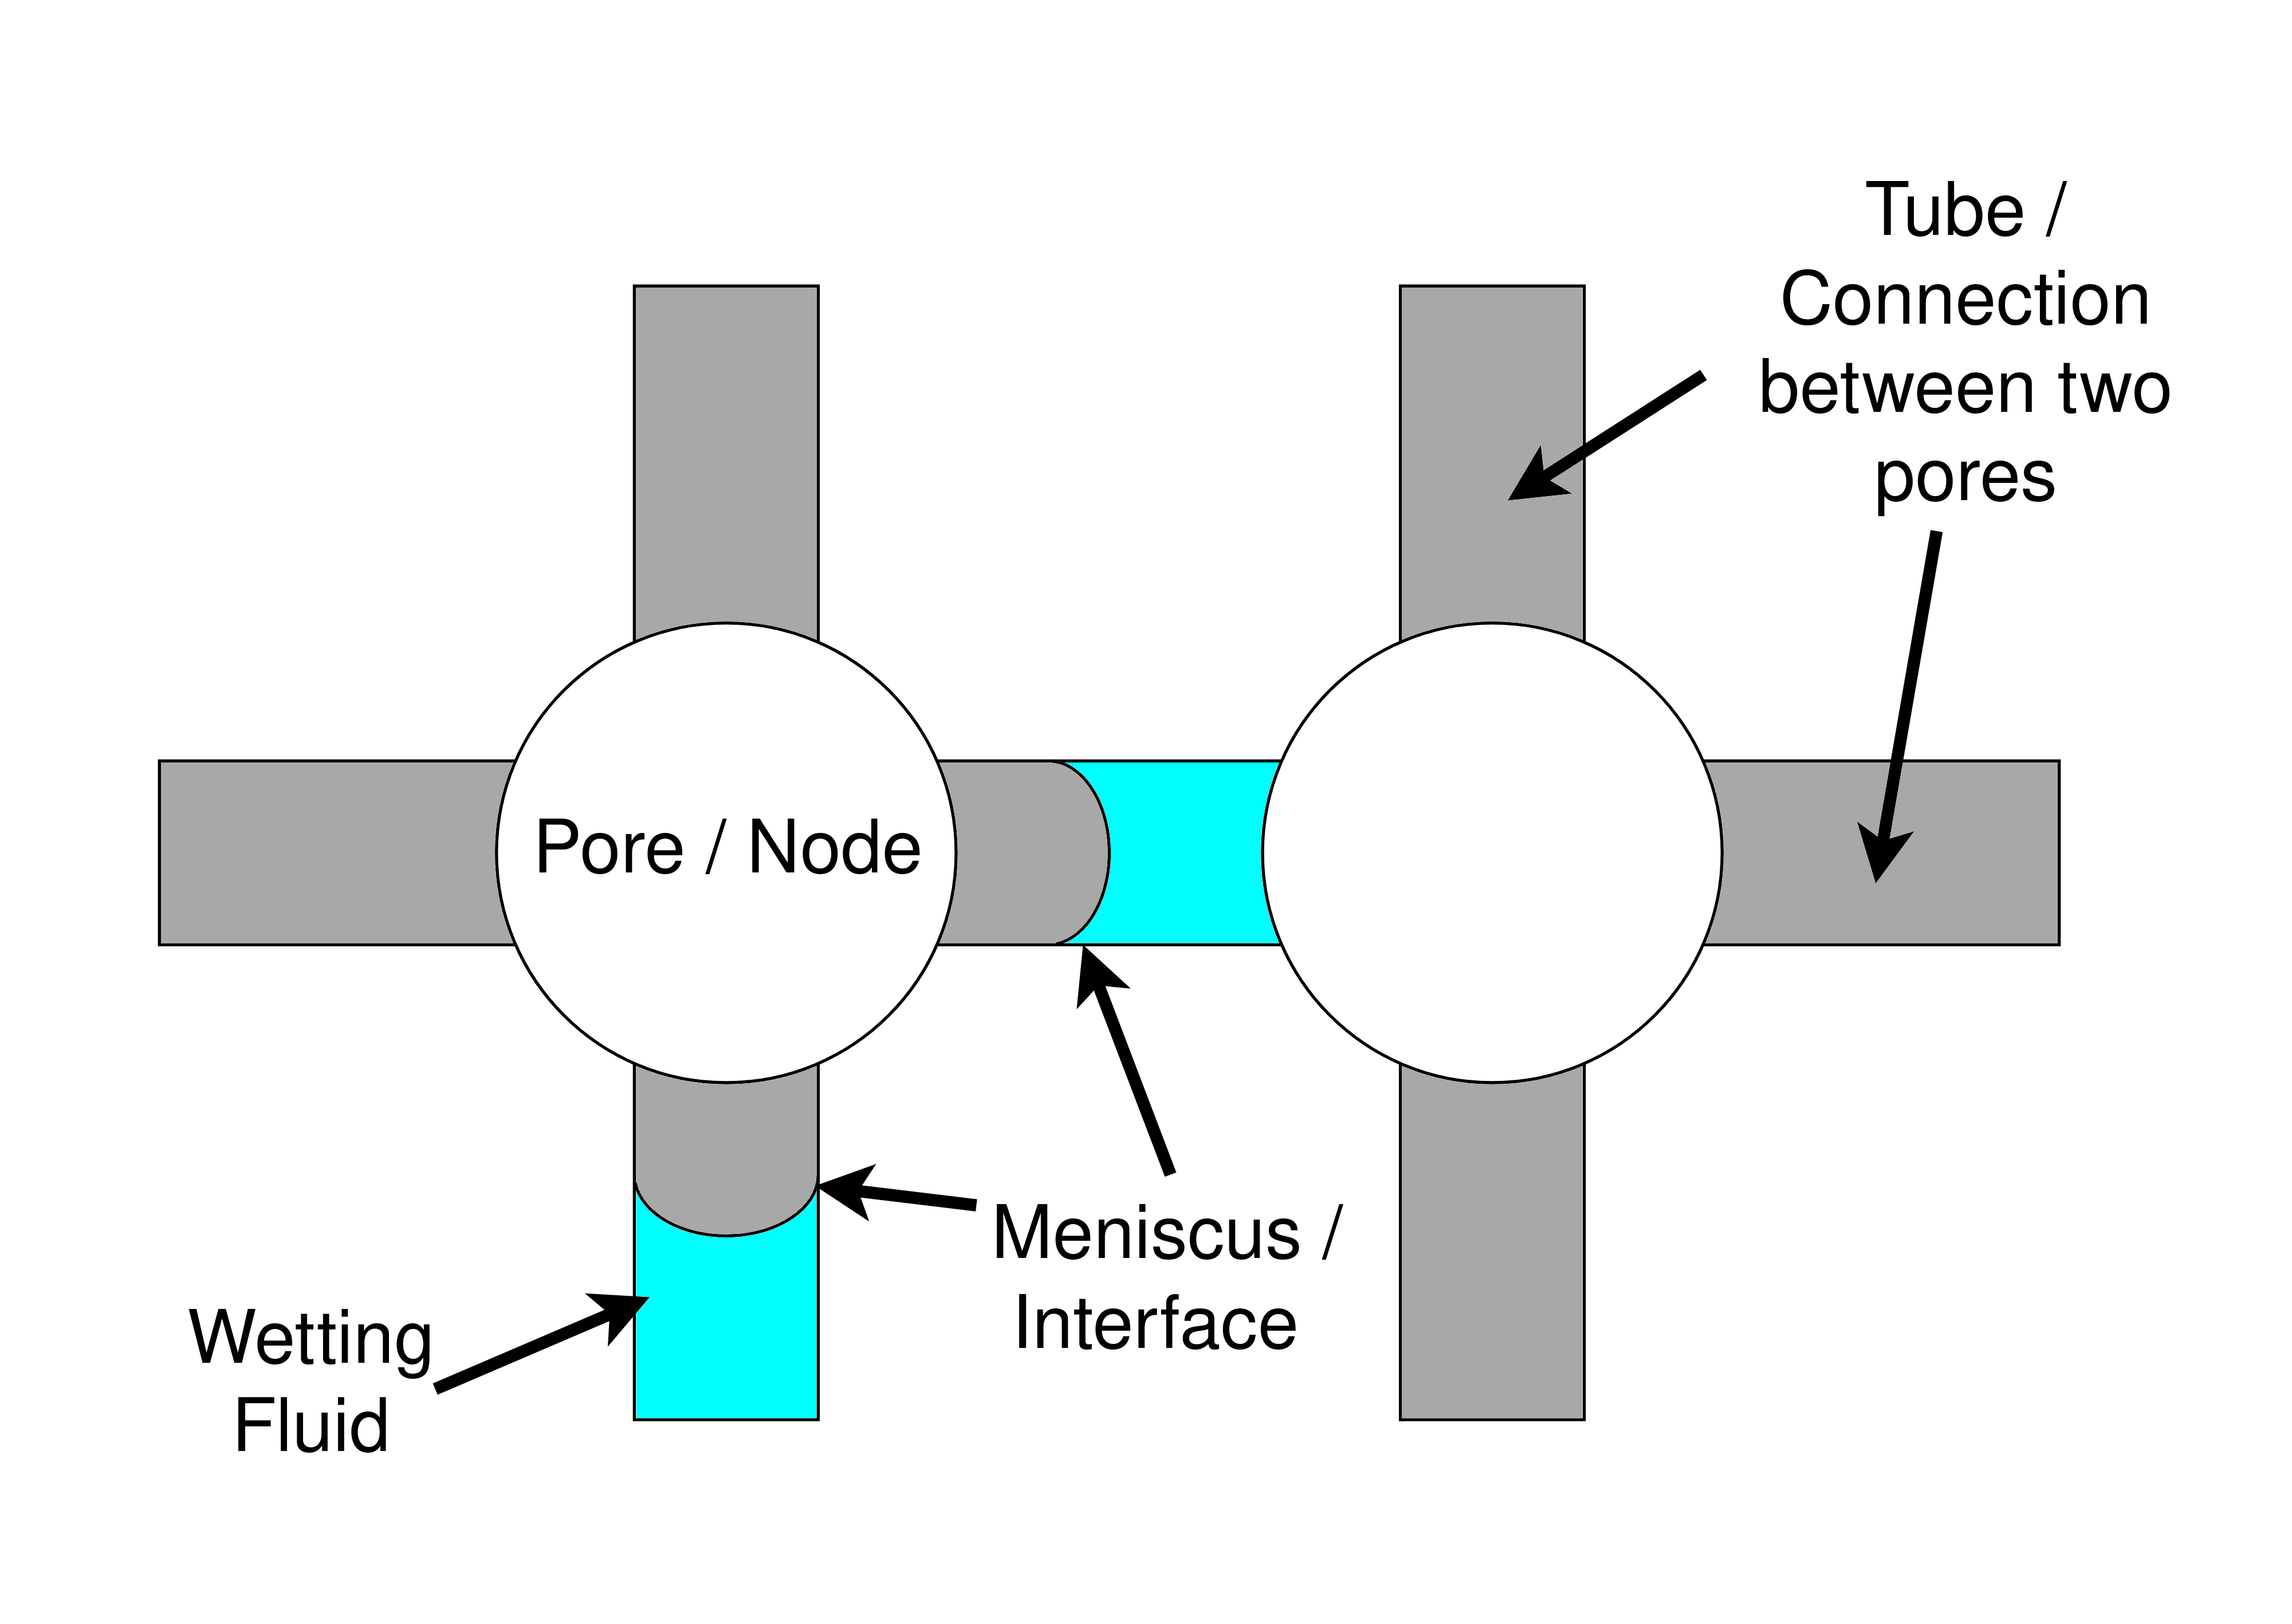
\includegraphics[height=6cm]{fig_descp-of-model}
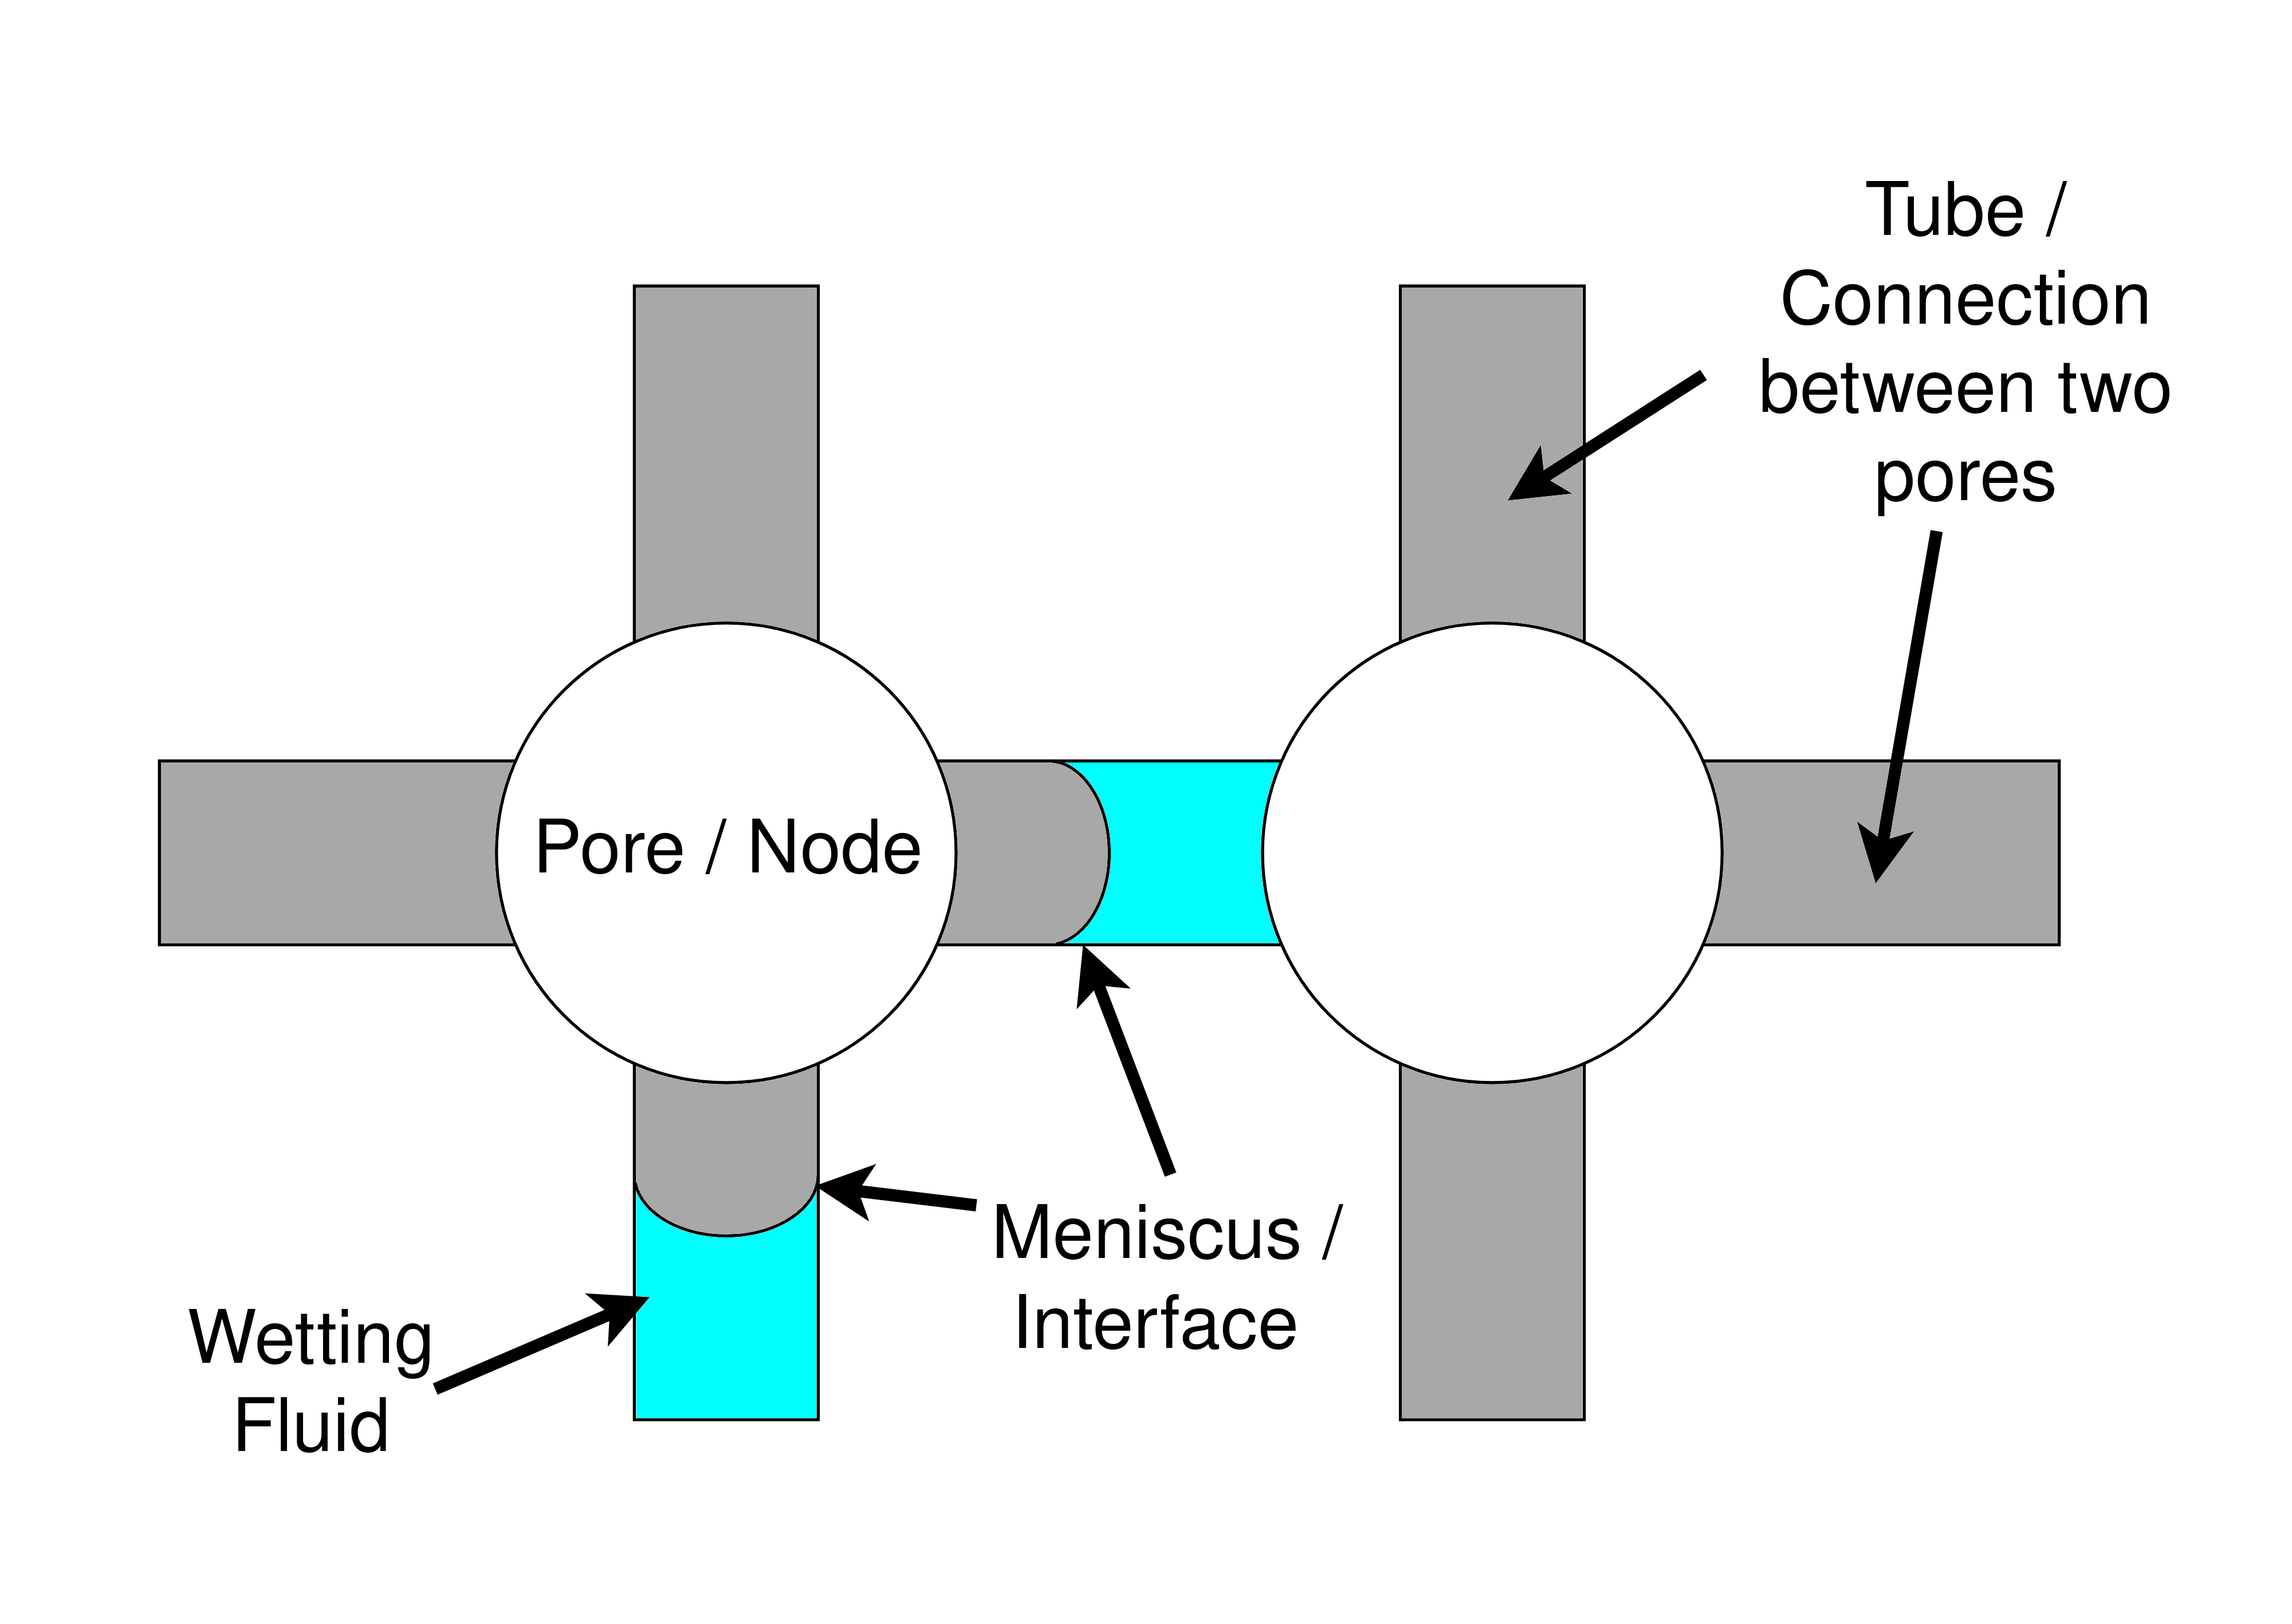
\includegraphics[height=6cm]{fig_descp-of-model}
Our model is initially set up such that the wetting fluid is low in saturation and is confined to the bottom of our network. A higher pressure is fixed for all nodes at the bottom layer, while a  low pressure is fixed for the top row. In all nodes, law of conservation of volume is applied, since mass is conserved and the phases are non-compressible. However for the bottom layer of nodes, the wetting fluid is injected as much required according to the sum of flow rates determined in the tubes connected to those nodes, while from the top layer of nodes a fluid is removed.
\section{Conclusion}
This algorithm can be extended to the case where there are more than 4 tube connections to a node, since for two phase flow into a node case, we distribute in an ascending order of radii, in our model it is distributed to a maximum number to two tubes, but for hexagonal model it can be 4. We only need to update the function which produces the connections. The same model can be used for a 3-dimensional case[2], where one surface has higher pressure than the opposite surface which has a lower pressure, it is to be used in order to more accurately represent the porous body.


\section{References}
\begin{enumerate}
	\item Aker, E., Måløy, K.J., Hansen, A., Batrouni, G.G. A two-dimensional network simulator for two-phase flow in porous media // Transp. Porous Med. 1998 V. 32 P. 163 
	\item Raoof A., Hassanizadeh S. A new method for generating pore-network models of porous media // Transp. Porous Med. 2010. V. 81. P. 391
	\item S. Sinha et al. Effective rheology of two-phase flow in three-dimensional porous media: experiment and simulation // Transp. Porous Med. 2017. V. 119. P. 77
	\item Fatt I. The network model of porous media 3, dynamic properties of networks with tube radius distribution Petroleum Trans. AIME 1956. V. 207. P. 164

\end{document}
